\documentclass[11pt,a4paper]{article}
\usepackage[utf8]{inputenc}
\usepackage[T1]{fontenc}
\usepackage[a4paper,margin=1in]{geometry}
\usepackage{lmodern}
\usepackage{amsmath,amssymb,mathtools}
\usepackage{graphicx}
\usepackage{caption}
\usepackage{subcaption}
\usepackage{enumitem}
\usepackage{hyperref}
\usepackage{booktabs}
\usepackage{microtype}
\usepackage{xcolor}
\usepackage{tcolorbox}
\usepackage{float}

% Tighter spacing for sections
\usepackage{titlesec}
\titlespacing*{\section}{0pt}{1.2ex plus 0.8ex minus .2ex}{0.8ex plus .2ex}
\titlespacing*{\subsection}{0pt}{0.9ex plus 0.6ex minus .2ex}{0.5ex plus .2ex}

% Global compactness (form only)
\setlength{\parindent}{0pt}
\setlength{\parskip}{0.35em}
\setlength{\textfloatsep}{10pt plus 2pt minus 2pt}
\setlength{\floatsep}{8pt plus 2pt minus 2pt}
\setlength{\intextsep}{8pt plus 2pt minus 2pt}
\setlength{\abovedisplayskip}{7pt plus 2pt minus 2pt}
\setlength{\belowdisplayskip}{7pt plus 2pt minus 2pt}
\setlength{\abovecaptionskip}{4pt}
\setlength{\belowcaptionskip}{0pt}

\title{\textbf{From Denoising to Scores: DAEs to Noise-Conditional Score Networks}}
\author{Ilan Aliouchouche \and Clément Marie \and Karim Rochd}
\date{ENS Paris-Saclay - Master MVA, 2025}

\begin{document}

\maketitle

\begin{abstract}
This report explores the theoretical evolution of generative modeling from Energy-Based Models to modern Score-Based methods. We analyze the connection established by Vincent (2011) between Denoising Autoencoders and Score Matching, and examine how Song \& Ermon (2019) leveraged this insight to address the manifold hypothesis using Noise-Conditional Score Networks and Annealed Langevin Dynamics.
\end{abstract}

\begin{center}
\small
\textbf{Code:} \href{https://github.com/karimrochd/MVA_PGM/tree/main}{github.com/karimrochd/MVA\_PGM}
\end{center}
\vspace{0.5em}

\section*{Author Contributions}
\begin{itemize}[noitemsep,leftmargin=*]
  \item \textbf{Ilan Aliouchouche:} Developed the theoretical background on energy-based models and score matching, detailed the Vincent (2011) DAE–DSM connection, selected and derived key equations, and drafted the \emph{Background} and \emph{Vincent (2011)} sections. Implemented a DAE trained on 1D manifolds to visualize and analyze the learned score fields.
  \item \textbf{Karim Rochd:} Presented and analyzed the Song \& Ermon (2019) framework, including noise-conditioning and annealed Langevin dynamics. Contributed to the interpretation of experimental limitations and authored the \emph{Discussion \& Limitations} and \emph{Conclusion} sections.
  \item \textbf{Clément Marie:} Implemented the DAE and NCSN architectures and training pipelines, developed Langevin and annealed Langevin samplers, designed and conducted the experiments (toy data and MNIST), and wrote the \emph{Experimental Results} section.
\end{itemize}

% ========================
\section{Introduction}

Generative modeling aims to learn the underlying probability distribution $p_{\text{data}}(x)$ of a dataset. While likelihood-based methods and implicit models (GANs) have dominated the field, Energy-Based Models (EBMs) offer a flexible alternative by modeling the density up to a normalizing constant. However, EBMs historically faced a significant bottleneck: the intractability of the partition function. To bypass this, Hyvärinen proposed \textit{Score Matching}, shifting the objective from estimating the density itself to estimating its gradient (the score) \cite{hyvarinen2005}.

This report analyzes two papers that bridged heuristic feature learning and principled probabilistic modeling. First, \textbf{Vincent (2011)} \cite{vincent2011} showed that Denoising Autoencoders (DAEs) are mathematically equivalent to performing score matching on a noise-smoothed data distribution. Building on this, \textbf{Song \& Ermon (2019)} \cite{song2019} identified limitations in applying standard score matching to high-dimensional data, specifically the manifold hypothesis. They introduced \textit{Noise-Conditional Score Networks} (NCSN) combined with annealed Langevin dynamics, a framework that leverages the DAE-score connection to achieve state-of-the-art generative performance.

\paragraph{Notation (used throughout).}
We denote by $p_{\text{data}}(x)$ the unknown data distribution of clean samples $x$.
A corruption process is written $q(\tilde{x}\mid x)$, where $\tilde{x}$ is a noisy version of $x$ (e.g. $\tilde{x}=x+\varepsilon$).
The resulting \emph{marginal} noisy distribution at scale $\sigma$ is
$q_\sigma(\tilde{x})=\int q_\sigma(\tilde{x}\mid x)\,p_{\text{data}}(x)\,dx$.
We call $\nabla_{\tilde{x}}\log q_\sigma(\tilde{x})$ the \emph{score} of the smoothed density at noise level $\sigma$.



% ========================
\section{Background}

\subsection{Energy-Based Models and Score Matching}

Energy-based models define a probability density
\[
p_\theta(x) = \frac{1}{Z_\theta}\exp(-E_\theta(x)),
\]
where the normalizing constant $Z_\theta$ is generally intractable. To avoid computing $Z_\theta$, Hyvärinen (2005) introduced \textbf{score matching}, which minimizes the distance between the model score $\psi_\theta(x) = \nabla_x \log p_\theta(x)$ and the data score $\psi_{\text{data}}(x) = \nabla_x \log p_{\text{data}}(x)$. The \textit{Explicit Score Matching} (ESM) objective is:
\[
J_{\text{ESM}}(\theta) = \frac{1}{2} \mathbb{E}_{p_{\text{data}}(x)} \left[ \left\| \psi_\theta(x) - \psi_{\text{data}}(x) \right\|^2 \right].
\]
Since $\psi_{\text{data}}(x)$ is unknown, Hyvärinen derived an equivalent \textit{Implicit Score Matching} (ISM) objective \cite{hyvarinen2005} using integration by parts, which depends only on the model's energy function and data samples.

\subsection{Denoising Autoencoders (DAEs)}

Denoising Autoencoders are neural networks trained to reconstruct a clean input $x$ from a corrupted version $\tilde{x} \sim q(\tilde{x}|x)$. A common choice is additive Gaussian noise $\tilde{x} = x + \varepsilon$, with $\varepsilon \sim \mathcal{N}(0, \sigma^2 I)$. Let $f_\theta$ be an encoder and $g_\theta$ a decoder.

\begin{tcolorbox}[colback=gray!5!white,colframe=black,left=2pt,right=2pt,top=2pt,bottom=2pt, title={DAE Training Objective}]
The DAE minimizes the expected reconstruction error (typically squared Euclidean norm):
\begin{equation}
    \mathcal{L}_{\text{DAE}}(\theta) = \mathbb{E}_{x \sim p_{\text{data}}} \mathbb{E}_{\tilde{x} \sim q(\tilde{x}|x)} \left[ \left\| g_\theta(f_\theta(\tilde{x})) - x \right\|^2 \right].
\end{equation}
\end{tcolorbox}

Intuitively, the DAE learns a vector field pointing from the noisy observation $\tilde{x}$ back toward the data manifold. As we will see, Vincent (2011) proved that this reconstruction vector is proportional to the score of the smoothed density.

% ========================
\section{Vincent (2011): Denoising Autoencoders are Score Matchers}

Vincent (2011) established a link between heuristic Denoising Autoencoders (DAEs) and probabilistic score matching \cite{vincent2011}. Training a DAE to denoise samples is mathematically equivalent to estimating the score of the data distribution smoothed by the corruption noise.

\subsection{Denoising Score Matching (DSM)}

Standard score matching requires the intractable data score $\nabla_x \log q(x)$ \cite{hyvarinen2005}. To bypass this, Vincent introduced \textbf{Denoising Score Matching (DSM)}, which matches the score of a conditional corruption distribution $q(\tilde{x}|x)$. Given a clean sample $x$ and a corrupted version $\tilde{x} \sim q(\tilde{x}|x)$, the DSM objective is defined as:
\begin{equation}
    J_{\mathrm{DSM}}(\theta) = \frac{1}{2} \mathbb{E}_{q(x, \tilde{x})} \left[ \left\| \psi(\tilde{x};\theta) - \nabla_{\tilde{x}} \log q(\tilde{x}|x) \right\|^2 \right].
\end{equation}
Crucially, the target $\nabla_{\tilde{x}} \log q(\tilde{x}|x)$ is analytically tractable. For Gaussian corruption $\tilde{x} = x + \varepsilon$ with $\varepsilon \sim \mathcal{N}(0,\sigma^2 I)$, the conditional density satisfies
\[
\nabla_{\tilde{x}} \log q(\tilde{x}\mid x)
= \frac{x - \tilde{x}}{\sigma^2}.
\]

The optimal score model $\psi^*$ minimizing $J_{\mathrm{DSM}}$ is the conditional expectation of this target \cite{vincent2011}:
\begin{equation}
    \psi^*(\tilde{x}) = \mathbb{E}_{q(x|\tilde{x})} \left[ \frac{x - \tilde{x}}{\sigma^2} \right] = \frac{1}{\sigma^2} \left( \underbrace{\mathbb{E}[x|\tilde{x}]}_{\text{Optimal Denoising}} - \tilde{x} \right).
    \label{eq:optimal_score}
\end{equation}
Equation (\ref{eq:optimal_score}) reveals the geometric interpretation: the optimal score field corresponds to the vector pointing from the noisy point $\tilde{x}$ back towards the clean data manifold.

\begin{figure}[H]
    \centering
    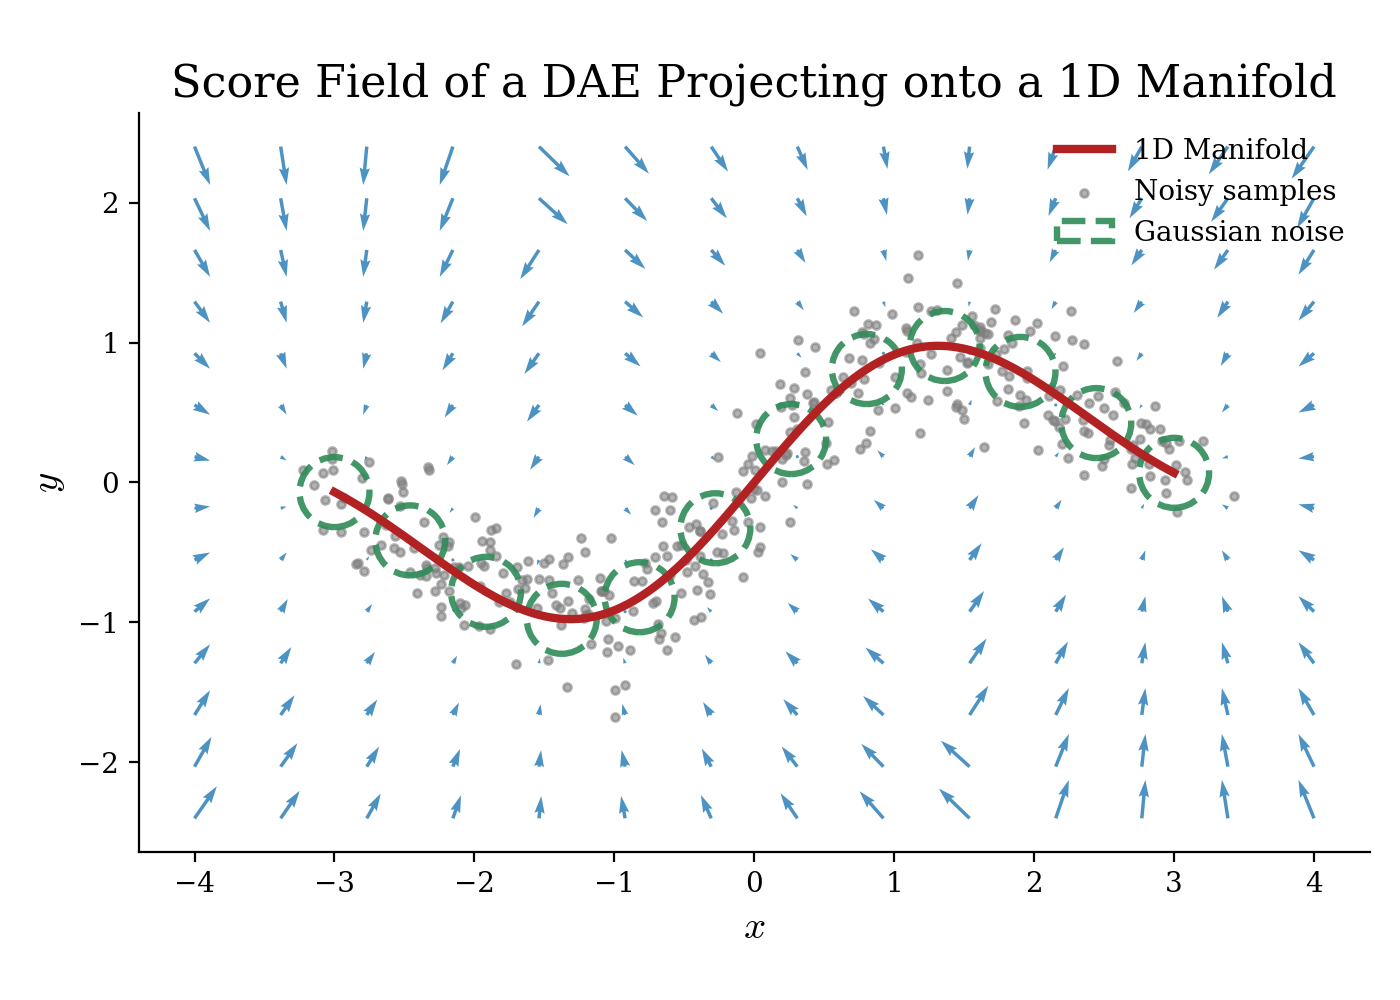
\includegraphics[width=0.45\textwidth]{scores.png}
    \caption{\small Visualization of the learned vector field. Blue arrows represent the score $\psi(\tilde{x})$, pointing from noisy samples (grey) back towards the high-density data manifold (red).}
    \label{fig:scores_fig}
\end{figure}

\subsection{Equivalence with the DAE Objective}

Vincent (2011) shows that, for a particular parametrization, the denoising score matching (DSM) objective coincides with the standard DAE reconstruction objective, up to a constant factor \cite{vincent2011}.

\begin{tcolorbox}[colback=gray!5!white,colframe=black,title={Theorem: DSM $\equiv$ DAE (Vincent, 2011)}, left=2pt,right=2pt,top=2pt,bottom=2pt]
Consider a Gaussian-corruption DAE with a single hidden layer and tied weights $W$. The hidden nonlinearity is the \emph{sigmoid} function, denoted $\mathrm{sigm}(\cdot)$, and the associated energy involves the \emph{softplus} function $\operatorname{softplus}(u)=\log(1+e^{u})$, whose derivative is $\nabla \operatorname{softplus}(u)=\mathrm{sigm}(u)$.
Define the energy-based model
\[
E(x;\theta) \;=\; -\frac{1}{\sigma^{2}}\left(\langle c, x\rangle - \frac{1}{2}\|x\|^{2} + \sum_{j}\operatorname{softplus}\!\big(\langle W_{j}, x\rangle + b_{j}\big)\right),
\]
where $\theta=(W,b,c)$. Its score is
\[
\psi(x;\theta) \;=\; \nabla_x \log p_\theta(x)
\;=\; \frac{1}{\sigma^{2}}\Big(W^{\top}\mathrm{sigm}(Wx+b) + c - x\Big).
\]
Substituting this parametrization into the DSM objective with Gaussian corruption yields a proportionality with the DAE squared reconstruction loss $L_{\mathrm{DAE}}$ \cite{vincent2011}:
\begin{equation}
J_{\mathrm{DSM}}(\theta) \;=\; \frac{1}{2\sigma^{4}}\,L_{\mathrm{DAE}}(\theta).
\end{equation}
\end{tcolorbox}

\textbf{Conclusion:} Minimizing the DAE reconstruction loss is equivalent, up to a constant factor, to denoising score matching on the noise-smoothed density $q_\sigma(\tilde{x})$. Consequently, the learned denoising vector field $\mathbb{E}[x\mid \tilde{x}] - \tilde{x}$ is proportional to the score, and the noise level $\sigma$ controls the smoothing scale.

% ========================
\section{Song \& Ermon (2019): Noise-Conditional Score Networks}

\subsection{Motivation: the manifold and low-density problems}

Although Vincent (2011) showed that denoising autoencoders learn the score of a smoothed data distribution, using a single fixed noise level $\sigma$ remains insufficient for high-dimensional generative modeling. Real-world data, such as natural images, lie near a low-dimensional manifold in $\mathbb{R}^d$, where the score $\nabla_x \log p_{\text{data}}(x)$ is unstable in low-density regions. When sampling with Langevin dynamics, the estimated gradients outside the data support are unreliable, causing poor mixing \cite{song2019}.

To address this, Song and Ermon (2019) proposed to train the score network across multiple noise levels, making the data distribution well behaved over all of $\mathbb{R}^d$.

\subsection{Noise-conditional network formulation}

The key idea is to make the score model explicitly depend on the noise level $\sigma$. Let $\{\sigma_1 > \sigma_2 > \cdots > \sigma_L\}$ denote a geometric sequence of noise scales. The authors introduced a single model $s_\theta(x,\sigma)$ that receives both the noisy input $x$ and the noise level $\sigma$ as arguments:
\[
s_\theta(x,\sigma) \approx \nabla_x \log q_\sigma(x).
\]

\begin{tcolorbox}[colback=gray!5!white,colframe=black, title={Noise-Conditional Score Network (NCSN)}]
Given a ladder of noise scales $\{\sigma_i\}_{i=1}^{L}$, a single neural network $s_\theta(x,\sigma)$ is trained to estimate the scores using a weighted objective:
\begin{equation}
\mathcal L(\theta) =\frac{1}{L}\sum_{i=1}^{L} \lambda(\sigma_i) \cdot \ell(\theta;\sigma_i),
\label{eq:dsm-multi}
\end{equation}
where $\ell(\theta;\sigma_i)$ is the DSM loss. The paper establishes that $\lambda(\sigma_i) = \sigma_i^2$ is the \textbf{optimal weighting} to ensure the loss terms have the same magnitude across all scales \cite{song2019}.
\end{tcolorbox}

\subsection{Sampling with Annealed Langevin Dynamics}

Sampling uses \emph{Annealed Langevin Dynamics}, summarized below.

\begin{tcolorbox}[colback=gray!5!white,colframe=black, title={Algorithm: Annealed Langevin Dynamics}]
\begin{enumerate}[leftmargin=*,noitemsep]
  \item Initialize $x_0 \sim \mathcal{N}(0, \sigma_1^2 I)$.
  \item \textbf{for} $i = 1, \dots, L$ \textbf{do}
  \item \quad Set step size $\alpha_i = \epsilon \cdot (\sigma_i / \sigma_L)^2$.
  \item \quad \textbf{for} $t = 1, \dots, T$ \textbf{do}
  \item \quad \quad $x_{t+1} \leftarrow x_t + \frac{\alpha_i}{2} s_\theta(x_t,\sigma_i) + \sqrt{\alpha_i} z_t$, with $z_t \sim \mathcal{N}(0,I)$.
  \end{enumerate}
\end{tcolorbox}

% ========================
\section{Experimental Results and Observations}

To validate the theoretical connections, we conducted experiments on both 2D toy data and the MNIST dataset.

\subsection{Implementation Details (Reproducibility)}

\begin{table}[H]
\centering
\small
\setlength{\tabcolsep}{6pt}
\renewcommand{\arraystretch}{1.15}
\begin{tabular}{@{}p{0.26\textwidth} p{0.68\textwidth}@{}}
\toprule
\textbf{Component} & \textbf{Setting} \\
\midrule
Data & MNIST, normalized to $[-1,1]$. No augmentation. \\
Optimizer & Adam, learning rate $10^{-3}$, batch size 64, 50 epochs. \\
Architecture & ScoreUNet; conditioning by concatenating a $\sigma$-map channel; output scaling by $1/\sigma$. \\
Noise schedule (Ablation) & Geometric ladder from $\sigma_1=10$ to $\sigma_L=0.01$, with $L\in\{1,10,50\}$. \\
Noise schedule (Bridge) & Geometric ladder from $\sigma_1=5$ to $\sigma_L=0.01$, with $L=10$. \\
Training objective & Denoising Score Matching (DSM) with weighting $\lambda(\sigma)=\sigma^2$. \\
Sampling (Annealed Langevin) & Step size $\alpha_i=\epsilon(\sigma_i/\sigma_L)^2$ with $\epsilon=2\cdot 10^{-5}$; $T=200$ for $L>1$, and $T=1000$ for $L=1$. \\
Baseline (Vincent DAE) & DAE trained with reconstruction MSE at $\sigma=0.1$; sampling with standard Langevin (1000 steps, step size $10^{-4}$). \\
\bottomrule
\end{tabular}
\caption{\textbf{Implementation details for reproducibility.} Summary of training, noise schedules, and sampling hyperparameters used in our experiments.}
\label{tab:impl_details}
\end{table}

% ========================
% TOY: MERGED FIGURE (VECTOR FIELD + MIXING)
% ========================
\subsection{Toy Experiment: Vector Field and Mixing}

We trained a DAE on a 2D Mixture of Gaussians (8 modes) and compare sampling with standard and annealed Langevin dynamics (Figure~\ref{fig:toy_merged}).

\begin{figure}[H]
\centering
\begin{subfigure}[t]{0.4\textwidth}
  \centering
  
\includegraphics[width=\textwidth]{exp1_vector_field.png}
  \caption{\textbf{Learned vector field.} DAE denoising directions align with the score field.}
  \label{fig:toy_vector_field}
\end{subfigure}\hfill
\begin{subfigure}[t]{0.55\textwidth}
  \centering
  
\includegraphics[width=\textwidth]{exp1_mixing_comparison.png}
  \caption{\textbf{Mixing comparison.} Annealed Langevin improves mode coverage vs standard Langevin.}
  \label{fig:toy_mixing}
\end{subfigure}
\caption{\textbf{Toy diagnostics (Mixture of Gaussians).} Left: DAE-learned denoising vectors approximate the score. Right: annealing mitigates poor mixing by traversing modes at high noise before refinement.}
\label{fig:toy_merged}
\end{figure}

% ========================
% MNIST: MERGED FIGURE (ABLATION + BRIDGE)
% ========================
\subsection{MNIST Experiments: Ablation and Bridge}

We scaled the approach to MNIST, studied the effect of the number of noise levels $L$, and report a bridge comparison between the Vincent-style DAE baseline and a multi-scale NCSN (Figure~\ref{fig:mnist_merged}).

\begin{figure}[H]
\centering
\begin{subfigure}[t]{0.7\textwidth}
  \centering
  
\includegraphics[width=\textwidth]{exp3_ablation_study_improved.png}
  \caption{\textbf{Ablation on $L$.} Best trade-off at $L=10$ under fixed sampling hyperparameters.}
  \label{fig:mnist_ablation}
\end{subfigure}\hfill
\begin{subfigure}[t]{0.7\textwidth}
  \centering
  
\includegraphics[width=\textwidth]{bridge_experiment_mnist.png}
  \caption{\textbf{Bridge experiment.} DAE + Langevin (left) vs NCSN + annealed Langevin (right).}
  \label{fig:mnist_bridge}
\end{subfigure}
\caption{\textbf{MNIST results (qualitative, $N=16$).}
Left: ablation over the number of noise levels $L$.
Right: bridge comparison between a single-noise Vincent DAE baseline and a multi-noise NCSN sampled with annealed Langevin.}

\label{fig:mnist_merged}
\end{figure}

\section{Discussion and Limitations}

\subsection{Quantitative Analysis: Smoothness versus Diversity}

We quantify the trade-off between \textbf{sample smoothness} and \textbf{sample diversity}.
Smoothness is measured by total variation (TV), while diversity is measured by the mean pairwise $\ell_2$ distance.
All metrics are computed on $N=256$ generated samples.

\paragraph{Metrics.}
We use \textbf{TV} to capture high-frequency artifacts, \textbf{pairwise $\ell_2$} as a diversity proxy, and
\textbf{saturation} as the fraction of near-clipped pixels
$\mathrm{Sat}(x)=\frac{1}{HW}\sum_{i,j}\mathbf{1}\{|x_{i,j}|\ge 0.95\}$ (averaged over samples).

\begin{table}[H]
    \centering
    \small
    \renewcommand{\arraystretch}{1.2}
    \begin{tabular}{@{}lccc@{}}
    \toprule
    \textbf{Method} & \textbf{TV} $\downarrow$ & \textbf{L2} $\uparrow$ & \textbf{Saturation} \\
    \midrule
    DAE (Vincent) & 1.515 & \textbf{27.73} & Low ($\sim 20\%$) \\
    NCSN ($L=1$) & 1.491 & 27.05 & Low ($\sim 16\%$) \\
    NCSN ($L=10$) & 0.251 & 21.41 & High ($\sim 69\%$) \\
    NCSN ($L=50$) & \textbf{0.160} & 15.46 & Very High ($\sim 77\%$) \\
    \bottomrule
    \end{tabular}
    \caption{\textbf{Smoothness--diversity trade-off.}
    Increasing $L$ reduces TV but also decreases diversity, revealing a trade-off between visual smoothness and mode coverage.}
    \label{tab:tradeoff}
\end{table}

\textbf{Observation.}
Single-noise models yield high diversity but strong high-frequency noise.
Multi-scale sampling reduces noise, while excessive annealing ($L=50$) lowers diversity and increases saturation.

\textbf{Conclusion.}
A moderate number of noise levels ($L=10$) provides the best compromise under fixed sampling hyperparameters.

\subsection{The Manifold Barrier}

Single-noise models fail when initialized far from the data manifold, where score estimates are unreliable.
This leads to unstable Langevin trajectories.

Noise-conditional models mitigate this by starting from large noise, where the density is smooth, and progressively refining samples toward the manifold.
Our results confirm this multi-scale strategy is essential in high dimensions.

\subsection{Computational Cost and Hyperparameter Sensitivity}

Score-based sampling requires $L\times T$ sequential score evaluations, making inference significantly slower than single-pass generators such as GANs or VAEs.

Moreover, annealed Langevin dynamics is sensitive to hyperparameters.
Increasing $L$ without retuning the step size $\epsilon$ can cause instability, emphasizing the practical cost of multi-scale score models.



\section{Conclusion}

The evolution from the Denoising Autoencoder (DAE) to the Noise-Conditional Score Network (NCSN) provides a mathematically rigorous foundation for score-based generative modeling. \textbf{Vincent (2011)} established the critical theoretical equivalence: training a DAE with reconstruction loss is equivalent to performing score estimation on the smoothed data density. This validation separated score-based methods from traditional likelihood or adversarial approaches.

\textbf{Song \& Ermon (2019)} built upon this by solving the practical challenges of high-dimensional data, primarily the manifold hypothesis and poor mixing under single-noise sampling, through the use of noise-conditioning and annealed Langevin dynamics. Ultimately, these works demonstrated that modeling the \textbf{gradient} (or direction) of the data distribution offers a highly effective and principled path to generate complex, high-fidelity samples. This confirms score estimation as a distinct and competitive third paradigm in modern generative AI.

% ========================
\begin{thebibliography}{9}

\bibitem{hyvarinen2005}
A. Hyvärinen, ``Estimation of non-normalized statistical models by score matching,'' \textit{Journal of Machine Learning Research}, vol. 6, pp. 695–709, 2005.

\bibitem{vincent2011}
P. Vincent, ``A Connection Between Score Matching and Denoising Autoencoders,'' \textit{Neural Computation}, vol. 23, no. 7, pp. 1661–1674, 2011.

\bibitem{song2019}
Y. Song and S. Ermon, ``Generative Modeling by Estimating Gradients of the Data Distribution,'' in \textit{Advances in Neural Information Processing Systems (NeurIPS)}, 2019.

\end{thebibliography}

\end{document}
